\documentclass[dvipdfmx,11pt,a4paper,oneside,openany]{jsbook}
\usepackage{package}
%\usepackage{a4wide}
\usepackage[dvipdfmx]{hyperref}
\usepackage{pxjahyper}
\usepackage{tikz}
\usetikzlibrary{intersections, calc, arrows.meta}


%\addtolength{\fullwidth}{1truemm} %全体の幅(ヘッダ部の幅)を既定値から26mm小さくする
\setlength{\textwidth}{\fullwidth}  %本文の幅(textwidth)を全体の幅(=ヘッダ部の幅)にそろえる
\setlength{\evensidemargin}{5truemm}   %偶数ページの左余白を10mm(+1インチ)にする
\setlength{\oddsidemargin}{5truemm}    %奇数ページの左余白を10mm(+1インチ)にする

%\title{}
%\author{}
%\date{\today}
\begin{document}
%\maketitle

%\tableofcontents

%\makeatletter
%\@addtoreset{equation}{section}
%\def\theequation{\thesection.\arabic{equation}}
%\makeatother
\newcommand{\ctext}[1]{\raise0.2ex\hbox{\textcircled{\scriptsize{#1}}}}

% 表示文字列を"図"から"Figure"へ
\renewcommand{\figurename}{Fig. }

% 図番号を"<章番号>.<図番号>" へ
\renewcommand{\thefigure}{\arabic{figure}}

\setcounter{chapter}{4}
\chapter{QUANTISATION OF STATIC SOLUTION}
\section{Introduction}
これまでの議論では波動方程式から始まり, ミンコフスキー空間やユークリッド空間において, 様々なLocalizeされた古典解を調べ, 場の古典論との対応関係を調べてきた. 本チャプターではこれまで見てきた古典解に対して, 新たに場の量子論との関係を議論していく. %実際, 古典的なミンコフスキー解を量子論の束縛状態や散乱理論に関連付けることができたり, 励起状態を記述できたりする.

最もシンプルな方法として2章でメインに扱ったような静的ソリトン解の量子化から始めていくが, それにあたっては場の古典論と場の量子論の違いを把握した上で, その対応関係を通して議論が展開されていく. そのためにそれぞれの性質と対応関係について下記に簡単にまとめておく.

\vspace{1cm}
\begin{tikzpicture}
    \draw (2.9,5.7)--(2.9,6.3)--(4.8,6.3)--(4.8,5.7)--(2.9,5.7);
    \draw (2.9,6) node[right]{場の古典論};
    \draw (10.5,5.7)--(10.5,6.3)--(12.4,6.3)--(12.4,5.7)--(10.5,5.7);
    \draw (10.5,6) node[right]{場の量子論};
    \draw (0,0)--(15.2,0);
    \draw (0,0)--(0,6)--(2.9,6);
    \draw (4.8,6)--(10.5,6);
    \draw (12.4,6)--(15.2,6);
    \draw (15.2,0)--(15.2,6);
    \draw[dashed] (7.52,0)--(7.52,6);
    \draw (0.1,5) node[right]{1. 場が\underline{\bf c-numberの関数で記述}される.};
    \draw (7.6,5) node[right]{1. 場が\underline{\bf q-number(演算子)の関数で記述}される.};
    \draw (0.1,4.2) node[right]{2. 古典系において複数の\underline{\bf 場の状態の区別が可能}.};
    \draw (7.6,4.2) node[right]{2. 量子系において複数の\underline{\bf 場の状態の区別が不可能}.};
    \draw (7.9,3.8) node[right]{\footnotesize{$\rightarrow$ ヒルベルト空間においてSchr\"{o}dinger方程式に従う状態}};
    \draw (8.3,3.5) node[right]{\footnotesize{ベクトルを用いて区別.}};
    \draw (0.1,2.7) node[right]{3. 場のダイナミクスは\underline{\bf 非線形偏微分方程式}で記述};
    \draw (0.5,2.3) node[right]{され, \underline{\bf 解はスカラー関数}として現れる.};
    \draw (7.6,2.7) node[right]{3. 場のダイナミクスは\underline{\bf Heisenberg方程式で記述}};
    \draw (8,2.3) node[right]{され, \underline{\bf 解は演算子の関数}として現れる.};
    \draw (0.1,1.5) node[right]{4. 実際の\underline{\bf 粒子(particle)の概念を適用しない}.};
    \draw (0.4,1.1) node[right]{\footnotesize{$\rightarrow$ 粒子"描像"を適用.}};
    \draw (7.6,1.5) node[right]{4. 実際の\underline{\bf 粒子(particle)の概念が適用できる}.};
    \draw (7.9,1.1) node[right]{\footnotesize{$\rightarrow$ 同時固有状態にハミルトニアンと運動量演算子を作用させ}};
    \draw (8.2,0.8) node[right]{\footnotesize{た時, $E^2-\bm{P}^2=M^2$の関係から一定値$M$を生じる.}};
\end{tikzpicture}

%これらの手法の選択は、調和振動子の問題にシュレディンガー微分方程式、ファインマン経路積分、ハイゼンベルグ整流器法のどれを使うかというように、好みの問題もあります。

\section{The central idea}
一次元のポテンシャル$V(x)$に従う単位質量の粒子を考え, 古典論と量子論の比較をしながら, 量子化の手順を説明していく.

\subsection{How to describe the particle in classical theory and quantum theory}
古典論において粒子を記述する際には運動方程式を用いて
\begin{align}
    \frac{\mathrm{d^2}x}{\mathrm{d^2}t}=-\frac{\mathrm{d}V}{\mathrm{d}x}
\end{align}
で与えられ, その運動は$x(t)$で記述される. 一方, 量子論では粒子を記述するのに, $x$を用いるのではなく, 粒子の各エネルギー固有値$E_n$に対して波動関数$\psi_n(x)$を用いて
\begin{align}
    H\psi_n(x)=\left(\frac{1}{2}\hat{p}^2+V(x)\right)\psi_n(x)=E_n\psi_n(x), \qquad \left(\hat{p}\equiv -i\hbar\frac{\partial}{\partial x}\right)
\end{align}
というようなSchr\"{o}dinger方程式に従って記述される. ではこの2つの記述それぞれについて調べたときにわかることを古典論と量子論で対応させながら見ていく.


\subsection{Comparison of classical theory and quantum theory}
図\ref{fig1}のような$x=a, b, c$に極値をもつポテンシャル$V(x)$を考えたとき, 粒子の運動はポテンシャルに沿って行われる事実から考えると, この静的解は
\begin{subequations}
    \begin{align}
        x(t) & =a\qquad \text{(安定)}\label{eq:5.3a} \\
        x(t) & =b \qquad \text{(不安定)}             \\
        x(t) & =c \qquad \text{(安定)}
    \end{align}
\end{subequations}
の3つとなる. そして$x=a$での解\eqref{eq:5.3a}が最も粒子のエネルギーが小さい状態であることから, 古典的な基底状態と呼べる.
\begin{align}
    E_0^{\text{cl}}=V(a)
\end{align}

\setcounter{figure}{8}
\begin{figure}[H]
    \centering
    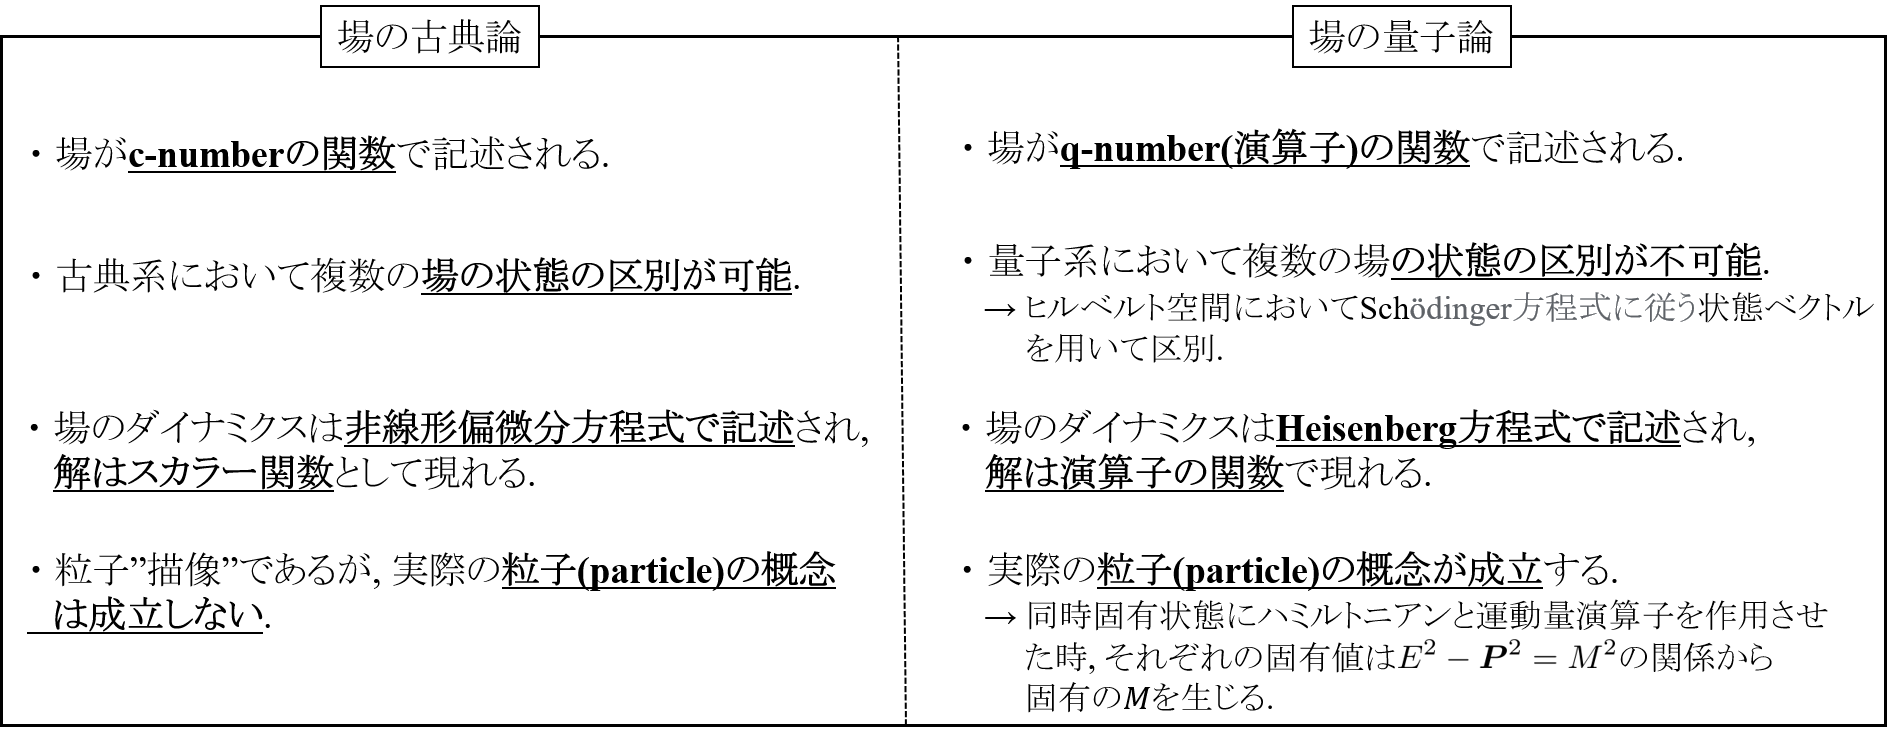
\includegraphics[width=7cm]{figure/fig1.png}
    \caption{}
    \label{fig1}
\end{figure}

では, 量子論ではどうかということを考えると, 不確定性原理から粒子の運動量または位置の変位がゼロに成ることはなく, 粒子の位置と運動は必ず揺らいでいる. 実際, 先のポテンシャルの基底状態であっても
\begin{align}
    E_0=E_{0}^{\text{cl}}+\Delta_0=V(a)+\Delta_0
\end{align}
というように$x=a$付近でエネルギーはゆらぐ. このとき$x=a$まわりで粒子がわずかに振動している場合, ポテンシャル$V(x)$を弱結合展開(weak-coupling expansion)することができる. つまりテイラー展開で
\begin{align}
    V(x)=V(a)+\frac{1}{2}\omega^2(x-a)^2+\frac{1}{3!}\lambda_3(x-a)^3+\frac{1}{4!}\lambda_4(x-a)^4+\cdots
\end{align}
というように調和振動+ゆらぎという形で展開ができる. そして, $x=a$まわりの振動を記述するのは第1項と第2項であり, それ以降は振動とは関係のない量子的なゆらぎの項である. したがって, 各項の波動関数には
\begin{align}
    \lambda_r\braket{(x-a)^r} \ll \omega^2\braket{(x-a)^2}, \qquad r=3,4,\cdots
\end{align}
の関係が成立しており, 同時にエネルギー固有値は
\begin{align}
    E_n=V(a)+\left(n+\frac{1}{2}\right)\hbar\omega+\mathcal{O}(\lambda_r)
\end{align}
というように定まることがわかる. そして基底状態に関して言えば
\begin{align}
    E_0=V(a)+\frac{1}{2}\hbar\omega+\mathcal{O}(\lambda_r)\label{eq:5.9} \\
    \braket{x}=\int |\psi_0(x)|^2 \mathrm{d}x=a+\cdots
\end{align}
というようにweak-couplingを用いて表現でき, 古典論との関わりがよく見て取れる.

では, $x=c$における解についても調べてみると, 古典的なエネルギーは
\begin{align}
    \tilde{E}^{\text{cl}}=V(c)
\end{align}
となり, $x=a$の場合と同様に調和振動のweak-coupling近似を行えば
\begin{align}
     & V(x)=V(c)+\frac{1}{2}(\omega')^2(x-c)^2+\sum_{r=3}\frac{\lambda'_r}{r!}(x-c)^r
\end{align}
\begin{subequations}
    \begin{align}
         & \tilde{E}_{n'}=V(c)+\hbar\omega'\left(n'+\frac{1}{2}\right)+\mathcal{O}(\lambda'_r) \\
         & \tilde{E}_{0}=V(c)+\frac{1}{2}\hbar\omega'+\mathcal{O}(\lambda'_r)
    \end{align}
\end{subequations}
\begin{align}
     & \braket{x}=c+\mathcal{O}(\lambda'_r)
\end{align}
というように表現することができる. しかしながらここで注視すべきことは, いま見ている状況設定では粒子にとって$x=c$付近での調和振動のみを考えており, 他のポテンシャル井戸の寄与はないとしていることである. 量子論においてはトンネル効果が成立することから$x=a$と$x=c$の互いのポテンシャル井戸を移動するということが起こり, 描像において2つの極値を行き来して混在することも考えうる. そこで, $\lambda_r$と$\lambda'_r$の値が共に小さければ互いのポテンシャルが一致することはなくなり, $x=a$と$x=c$は大きく離れ, ポテンシャル壁が存在することになる. このことにより, トンネリングを無視することができ, $x=a$と$x=c$における描像をそれぞれ別に考えることができるとして議論を進めていく.
%基底状態に関するすべての情報は、その波動関数に含まれています。しかし、古典解は、同じ近似において、基底状態の波動関数の他の特徴も与える。この基本的な理由は、この波動関数phi0がxに広がりを持っていても、古典解x=aの周りに典型的に局在するということです。例えば、その位置期待値は次のように与えられる。a+bここで、ドットは非調和定数lmabdaによる補正を表しています。ここで、(5.10)のaは単なる数字ですが、(5.3a)の静的な古典解を表しており、一方、左辺は量子基底状態の特性を表しています
%しかし、lambda_rとlambda'_rがすべて小さければ、2つの極小点x=aとx=cは大きく離れ、その間には大きな電位障壁が存在します。そのため、トンネリングは遅くなり、結果的にトンネリングによるエネルギー固有値の変化は、パラメータlambda_rとlambda'_rにおいて非摂動的な現象となる。弱結合展開の任意の有限オーダーにおいて、x=c付近の準位のセット(5.13)は、x=a付近のセット(5.8)とは別に考えることができる。


では, $N$個の粒子の$N$次元系での議論に拡張する. このときこれまでと同様にweak-coupling expansionを行えば, そのポテンシャル$V(x_1,x_2,\cdots,x_N)$は$x_i=a_i$周りにおいて
\setcounter{equation}{15}
\begin{align}
    \begin{aligned}
        V(x)= & V(\bm{a})+\frac{1}{2}\left(x_{i}-a_{i}\right)\left(x_{j}-a_{j}\right)\left[\frac{\partial^{2} V}{\partial x_{i} \partial x_{j}}\right]_{x=a}                                       \\
              & +\frac{1}{3 !}\left(x_{i}-a_{i}\right)\left(x_{j}-a_{j}\right)\left(x_{k}-a_{k}\right)\left[\frac{\partial^{3} V}{\partial x_{i} \partial x_{j} \partial x_k} \right]_{x=a}+\cdots
    \end{aligned}
\end{align}
というように展開することができる. そしてこれもまた量子論においては$x=a_i$周辺での調和振動の様子が見て取れるはずであり, そのモードおよび角振動数は第2項に含まれ, $\left(\dfrac{\partial^2 V}{\partial x_i\partial_j}\right)_{x=a}$の固有ベクトルと固有値$\omega_i^2$を求めれば自然と現れる. こういった背景から$\omega_i$を用いて$x=a$での基底状態におけるエネルギー及び各準位は
\begin{align}
    E_0=V(\bm{a})+\sum_{i=1}^{N}\frac{1}{2}\hbar\omega_i+\text{corrections} \\
    E_{\left\{n_{i}\right\}}=V(a)+\hbar \sum_{i=1}^{N}\left(n_{i}+\frac{1}{2}\right) \omega_{i}+\text { corrections. }
\end{align}
というように表すことができ, これもまた古典的配位(第1項)に量子的配位(第2項以降)を加えた形となっている.

ではさらに場の理論的立場から考察してみる, ラグランジアンを
\begin{align}
    L=\int \mathrm{d} x\left[\frac{1}{2}\left(\frac{\partial \phi}{\partial t}\right)^{2}-\frac{1}{2}(\boldsymbol{\nabla} \phi)^{2}-U(\phi)\right]\nonumber \\
    L=T[\phi]-V[\phi]
\end{align}
\begin{subequations}
    \begin{align}
        T[\phi]\equiv\frac{1}{2}\int \mathrm{d}x\left(\dfrac{\partial \phi}{\partial t}\right)^2 \\
        V[\phi] \equiv \int \mathrm{d} x\left[\frac{1}{2}(\nabla \phi)^{2}+U(\phi)\right]
    \end{align}
\end{subequations}
というように一般的な形で定義すれば, Euler-Lagrange方程式から導かれる運動方程式は
\begin{align}
    \frac{\partial^{2} \phi(x, t)}{\partial t^{2}}=-\frac{\delta V[\phi]}{\delta \phi(x, t)}
\end{align}
となり, 2章での議論と同様にニュートンの運動方程式との類似性が見て取れる. そして静的解という立場に戻れば
\begin{align}
    \dfrac{\delta V[\phi]}{\delta \phi(\bm{x})}=0
\end{align}
を満たす必要があり, そのような最小値を$\phi(\bm{x})=\phi_0(\bm{x})$とすればこれまでの方法と同様にTaylor展開をすれば
\begin{align}
    V[\phi]=V\left[\phi_{0}\right]+\int \mathrm{d} \bm{x} \frac{1}{2}\left\{\eta(\bm{x})\left[-\nabla^{2}+\left(\frac{\mathrm{d}^{2} U}{\mathrm{d} \phi^{2}}\right)_{\phi_{0}(\bm{x})}\right] \eta(\bm{x})+\cdots\right\}\label{eq:5.23} \\
    \qquad \left(\eta(\bm{x})\equiv \phi(\bm{x})-\phi_0(\bm{x})\right)\nonumber
\end{align}
としてポテンシャルを表現できる. ここで第2項はこれまでの議論でみてきた, 量子化したが故のゆらぎ, 調和振動を表現する項であるから, その項に対する固有値を求めれば振動の角振動数が定まる. つまり
\begin{align}
    \left[-\nabla^{2}+\left(\frac{\mathrm{d}^{2} U}{\mathrm{d} \phi^{2}}\right)_{\phi_{0}(x)}\right] \eta_{i}(x)=\omega_{i}^{2} \eta_{i}(x)\label{eq:5.24}
\end{align}
として量子化したときのモード$\eta$と角振動数$\omega_i$を定めることができる. ではこの$\eta(\bm{x},t)$を各モード$\phi_i$で書いて
\begin{align}
    \eta(x, t) & \equiv \phi(x, t)-\phi_{0}(x)\nonumber \\
               & \equiv \sum_{i} c_{i}(t) \eta_{i}(x)
\end{align}
としたとき, ラグランジアンはTaylor展開した\eqref{eq:5.23}を用いて
\begin{align}
    L=\frac{1}{2} \sum_{i}\left[\dot{c}_{i}(t)\right]^{2}-\left(V\left[\phi_{0}\right]+\frac{1}{2} \sum_{i}\left[c_{i}(t)\right]^{2} \omega_{i}^{2}\right)+\text { corrections }\label{eq:5.26} \\
    \qquad \left(\dot{c}_i\equiv \frac{\mathrm{d}c_i}{\mathrm{d}t}\right) \nonumber
\end{align}
というように変形できる. そして量子化した場合には古典的な項$V[\phi_0]$に対して調和振動の項とゆらぎの項が加わるという考えから, エネルギー準位は
\begin{align}
    E_{\left\{n_{i}\right\}}=V\left[\phi_{0}\right]+\hbar \sum_{i}\left(n_{i}+\frac{1}{2}\right) \omega_{i}+\text { corrections }\label{eq:5.27}
\end{align}
と書くことができる. ここで重要なのは\eqref{eq:5.24}, \eqref{eq:5.26}は単に古典的な安定性からポテンシャルをTaylor展開をしたものから導かれる関係式であり, そこから標準的な摂動の方法を用いて古典解から, 量子的なゆらぎの描像が現れているということである. なお, これまでの議論では$\omega_i$がゼロでないとする調和振動がゆらぎに関わっているものとしてきたが, もしそれがゼロとなる調和振動がないものに関してはポテンシャルの展開に関して少し改良を加える必要があるということに注意が必要である.

これまで見てきたのは古典的な真空解, つまり$\frac{\mathrm{d}V}{\mathrm{d}\phi}=0$となる$\phi_0$まわりでの通常の摂動論(weak;coupling)を考え, 量子的な情報を抽出した. これから我々がやりたいことは5章以前に扱ってきたキンクを始めとした様々な古典解を$\phi_0$として量子化することであり, 通常の摂動論は少し変化が生じる. これを一般的な$\phi^4$模型を用いて説明していく. ラグランジアンは
\begin{align}
    L       & =\int\mathrm{d}\bm{x}\left[\frac{1}{2}\left(\dfrac{\partial \phi}{\partial t}\right)^2-\frac{1}{2}m^2\phi^2+\frac{1}{4}\lambda\phi^4\right], \\
    V[\phi] & =\int\mathrm{d}\bm{x}\left[\frac{1}{2}\left(\nabla \phi\right)^2+\frac{1}{2}m^2\phi^2+\frac{1}{4}\lambda\phi^4\right]\nonumber               \\
            & =\int\mathrm{d}\bm{x}\left[-\frac{1}{2}\phi\nabla^2\phi+\frac{1}{2}m^2\phi^2+\frac{1}{4}\lambda\phi^4\right]\label{eq:5.29}
\end{align}
となり, Euler-Lagrange方程式から静的解は
\begin{align}
    \dfrac{\delta V[\phi]}{\delta \phi(\bm{x})}=-\nabla^2\phi+m^2\phi+\lambda\phi^3=0
\end{align}
に従う. \eqref{eq:5.29}のポテンシャルは
\begin{align}
    \phi_0(\bm{x},t)=0\qquad \text{with} \qquad V[\phi_0=0]=0
\end{align}
の$\phi_0$にて最小値ゼロをとっており, すでに$\phi_0$周りのTaylor展開の形となっていることがわかる. そこで, これまでの議論から$\phi=0$における二階微分の値を出すオペレーターは$(-\nabla^2+m^2)$に対応し, 固有値方程式は
\begin{align}
    \left(-\nabla^2+m^2\right)\eta_i(\bm{x})=\omega_i^2\eta_i(\bm{x})
\end{align}
となる. これを解けば
\begin{align*}
    \eta_i(x)=L^{-3/2}\exp\left(i\bm{k}_i\cdot \bm{x}\right) \\
    \qquad \left(\bm{k}_i=\frac{2\pi\bm{N}_i}{L}\right)
\end{align*}
となり, 分散関係は
\begin{align*}
    \omega_i^2=\bm{k}_i^2+m^2
\end{align*}
となる.(連続系にするためには$L\rightarrow\infty$をとれば良い.) そして今古典解に対して量子化したときの調和振動の角振動数が定まったことになるからエネルギーは
\begin{align}
    E_{\{n_i\}} & =V[\phi_0]+\hbar\sum_{k_i}\sqrt{k_i^2+m^2}\left(n_i+\frac{1}{2}\right)+\mathcal{O}(\lambda)\nonumber                      \\
                & =\hbar\sum_{k_i}\sqrt{k_i^2+m^2}\left(n_i+\frac{1}{2}\right)+\mathcal{O}(\lambda)\qquad \left(\because V[\phi_0]=0\right)
\end{align}
となり, 真空, そして次の励起は
\begin{align}
    E_{\mathrm{vac}} & \equiv E_{\{0\}}=\frac{1}{2} \hbar \sum_{k_{i}} \sqrt{k_{i}^{2}+m^{2}}+\mathcal{O}(\lambda)  \\
    E_{1}            & =\frac{1}{2} \hbar \sum_{k_{i}} \sqrt{k_{i}^{2}+m^{2}}+\hbar m+\mathcal{O}(\lambda)\nonumber \\
                     & =E_\text{vac}+\hbar m+\mathcal{O}(\lambda)
\end{align}
となる. ここで, 連続系であることから$k_i$のモードは無数に存在するため, エネルギーは発散するが, これはよく知られた事実である. この件については後のセクションで触れるとしてとりあえず今は$(E_{\{n_i\}}-E_\text{vac})$は有限になっているということは認識しておいてほしい.

\section{Quantisation of the kink solution}
これまでの方法を用いて実際に(1+1)次元のキンク解の量子化を行う. ラグランジアンは
\begin{align}
    L=\int \mathrm{d} x\left[\frac{1}{2}\left(\frac{\partial \phi}{\partial t}\right)^{2}-\frac{1}{2}\left(\frac{\partial \phi}{\partial x}\right)^{2}+\frac{1}{2} m^{2} \phi^{2}-\frac{\lambda}{4} \phi^{4}-\frac{m^{4}}{4 \lambda}\right]
\end{align}
とかけ, そのポテンシャルと関係式は2章で扱ったように
\begin{align}
    V[\phi]=\int \mathrm{d}x\left[\frac{1}{2}\left(\frac{\partial \phi}{\partial x}\right)^{2}+\frac{\lambda}{4}\left(\phi^{2}-\frac{m^{2}}{\lambda}\right)^{2}\right] \\
    \frac{\partial V[\phi]}{\partial \phi(x)}=-\frac{\partial^{2}}{\partial x^{2}} \phi-m^{2} \phi+\lambda \phi^{3}=0\label{eq:5.38}
\end{align}
となる. またその解は真空解(定常解)$\phi=\pm\frac{m}{\sqrt{\lambda}}$と$\phi_{K}(x, t)=\pm(m / \sqrt{\lambda})\tanh[m(x-a)/\sqrt{2}]$となる.

\subsubsection{The vacuum and its excitations}
まず$\phi_1(x,t)=m/\sqrt{\lambda}$の定常解の量子化を考える.これまで通り$\phi_1$周りの量子化を行えば
\begin{align}
    V[\phi] & =V[\phi_1]+\int \mathrm{d}x\left(-\frac{1}{2}\tilde{\phi}\dfrac{\partial^2\tilde{\phi}}{\partial x^2}-\frac{1}{2}m^2\tilde{\phi}^2+\frac{3}{2}\lambda\phi_1^2\tilde{\phi}^2\right)+\lambda\int\mathrm{d}x\left(\phi_1\tilde{\phi}^3+\frac{1}{4}\tilde{\phi}^4\right)\nonumber \\
            & = \int\mathrm{d}x\frac{\tilde{\phi}}{2}\left(-\dfrac{\partial^2}{\partial x^2}+2m^2\right)\tilde{\phi}+m\sqrt{\lambda}\int\tilde{\phi}^3\mathrm{d}x+\frac{\lambda}{4}\int\tilde{\phi}^4\mathrm{d}x                                                                            \\
            & \qquad\ \ \ \ \ \ \ \ \ \ \ \ \ \ \ \ \ \ \ \ \ \ \ \ \left(\tilde{\phi}(x)\equiv\phi(x)-\phi_1(x)=\phi(x)-\frac{m}{\sqrt{\lambda}}, \quad V[\phi_1]=0\right)\nonumber
\end{align}
となる. このことから量子化したときの調和振動を決めるオペレータは摂動展開したときの第2項で
\begin{align*}
    \left(-\dfrac{\partial^2}{\partial x^2}+2m^2\right)\tilde{\phi}=\omega^2\tilde{\phi}
\end{align*}
の固有値方程式を解けば良い. その結果
\begin{align}
    \omega^2=k_n^2+2m^2\nonumber    \\
    \tilde{\phi}=e^{ik_nx}\nonumber \\
    k_nL=2n\pi
\end{align}
を得る. もし連続系に拡張したければ境界条件から
\begin{align*}
    \sum_{k_{n}} \rightarrow \frac{L}{2 \pi} \int \mathrm{d} k
\end{align*}
という置き換えをすれば良い. このことから$\phi_1$まわりの真空エネルギー, 励起エネルギーは調和振動近似から
\begin{align}
    E_{\mathrm{vac}}=0+\frac{1}{2} h \sum_{n}\left(k_{n}^{2}+2 m^{2}\right)^{1 / 2}+\mathrm{O}(\lambda) \\
    E_{\{N_n\}}=\hbar \sum_{n}\left(N_{n}+\frac{1}{2}\right)\left(k_{n}^{2}+2 m^{2}\right)^{1 / 2}+\mathcal{O}(\lambda)\label{eq:5.42}
\end{align}
となる. またこれらは理論上量子に対応しており, $N_n$個の量子が運動量$\hbar k$, 静止質量$m\hbar \sqrt{2}$を持っていることがわかる. そしていま, $\lambda$が小さいとして摂動展開したのだから, $\tilde{\phi}=\phi-\phi_1$は$\phi=\phi_1$を中心として量子的な摂動をしていた$\phi$を$\phi_1$だけずらしたということになり真空状態の期待値は
\begin{align}
    \bra{0}\tilde{\phi(x,t)}\ket{0}=0
\end{align}
となり, 同時に
\begin{align}
    \bra{0}\phi(x,t)\ket{0}=\phi_1+\mathcal{O}(\lambda)
\end{align}
となる. 以上のように真空解周りの摂動展開を考えたときに得られる粒子(量子)はmesonと呼ばれている.(なお, 2つ真空があるが, もちろん別の真空にも同じ議論が適用され, $\bra{0}\phi(x,t)\ket{0}=\phi_2$が成立する. そしてこれらは$\phi\leftrightarrow-\phi$の対称性を破ることになり, これがまさに自発的対称性の破れと関係がある.)

\subsubsection{The quantum kink and its excitations}
ではキンク解
\begin{align}
    \phi_{K}(x-a)=\dfrac{m}{\sqrt{\lambda}} \tanh [\dfrac{m(x-a)}{\sqrt{2}}] \\
    V[\phi_{K}]=\dfrac{2\sqrt{2}}{3}\frac{m^3}{\lambda}
\end{align}
の量子化を同様の手順を踏んで考える. まず$a=0$とした場合, $\phi_K(x)$まわりの展開を考えると\eqref{eq:5.38}を用いて
\begin{align}
    V[\phi]=V\left[\phi_{K}\right]+\int \mathrm{d} x \frac{1}{2} \eta(x)\left(-\frac{\partial^{2}}{\partial x^{2}}-m^{2}+3 \lambda \phi_{K}^{2}\right) \eta(x)+\lambda\int\mathrm{d}x\left(\phi_{K}\eta^3+\frac{1}{4}\eta^4\right) \\
    \qquad \left(\eta(x)\equiv \phi(x)-\phi_{K}(x)\right)\nonumber
\end{align}
を得る. また$V[\phi]$の二階微分項から得られる固有値方程式は
\begin{align}
    \left(-\frac{\partial^{2}}{\partial x^{2}}-m^{2}+3 \lambda \phi_{K}^{2}\right) \eta_{n}(x) & =\left[-\frac{\partial^{2}}{\partial x^{2}}-m^{2}+3 m^{2} \tanh ^{2}\left(\frac{m x}{\sqrt{2}}\right)\right] \eta_{n}(x)\nonumber \\
                                                                                               & =\omega_n^2\eta_n(x)
\end{align}
となる. この方程式を解くために$z=\frac{mx}{\sqrt{2}}$とすれば
\begin{align}
    \left(-\frac{1}{2} \frac{\partial^{2}}{\partial z^{2}}+\left(3 \tanh ^{2} z-1\right)\right) \tilde{\eta}_{n}(z)=\frac{\omega_{n}^{2}}{m^{2}} \tilde{\eta}_{n}(z)
\end{align}
というようにSchr\"{o}dinger方程式と同じ形となり, その解は3つに限られ
\begin{subequations}
    \begin{align}
        \omega_{0}^{2}=0                                     & \text { with } \tilde{\eta}_{0}(z)=1 / \cosh ^{2} z                                                                                     \\
        \omega_{1}^{2}=\frac{3}{2} m^{2}                     & \text { with } \tilde{\eta}_{1}(z)=\sinh z / \cosh ^{2} z                                                                               \\
        \omega_{q}^{2}=m^{2}\left(\frac{1}{2} q^{2}+2\right) & \text{ with } \tilde{\eta}_{q}(z)=\mathrm{e}^{\mathrm{i} q z}\left(3 \tanh ^{2} z-1-q^{2}-3 \mathrm{i} q \tanh z\right)\label{eq:5.50c}
    \end{align}
\end{subequations}
となる.
\begin{figure}[H]
    \centering
    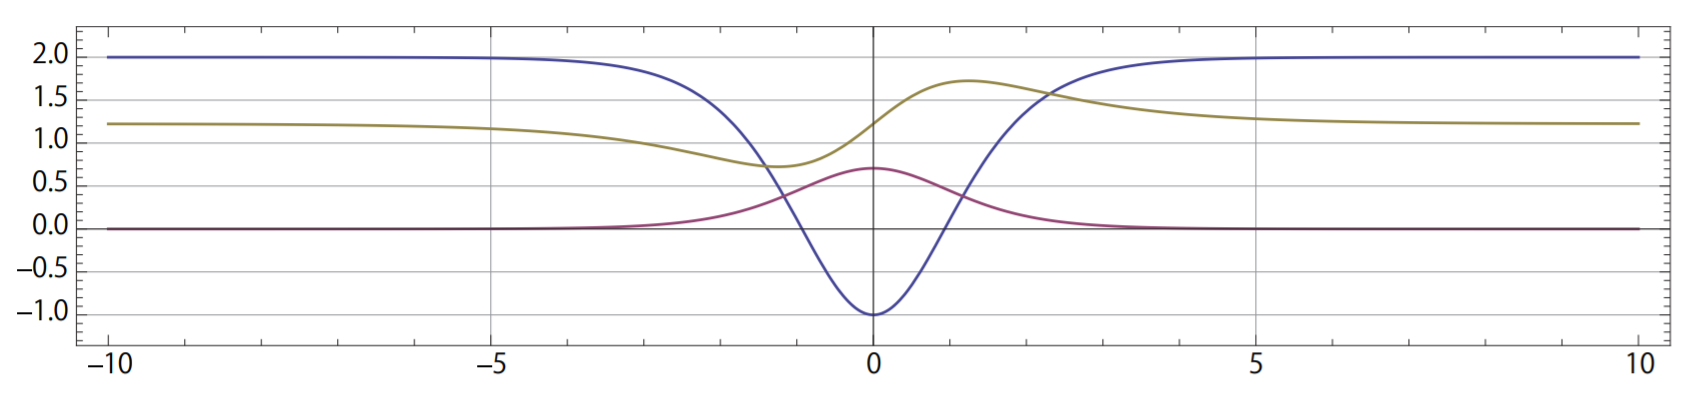
\includegraphics[width=12cm]{figure/fig3.png}
    \caption{ゼロモード}
    \label{fig3}
\end{figure}
\begin{figure}[H]
    \centering
    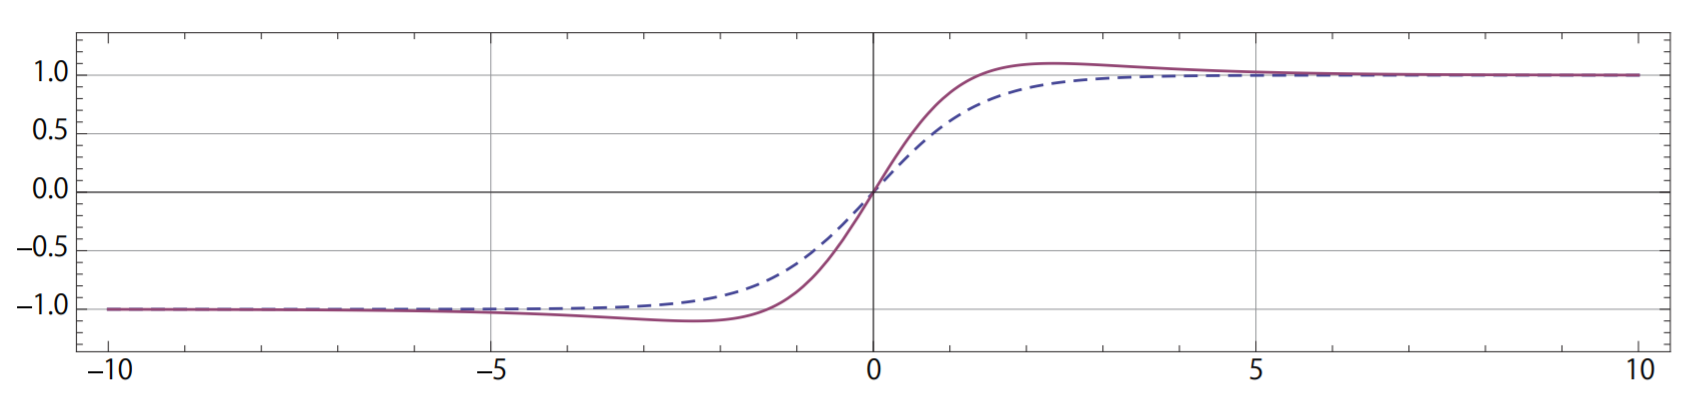
\includegraphics[width=12cm]{figure/fig4.png}
    \caption{変形モード}
    \label{fig3}
\end{figure}
ここで, \eqref{eq:5.50c}の$z\rightarrow\infty$での挙動については
\begin{align}
    \tilde{\eta}_{q}(z) \underset{z \rightarrow \pm \infty}{\longrightarrow} \exp \left[\mathrm{i}\left(q z \pm \frac{1}{2} \delta(q)\right)\right]\label{eq:5.51} \\
    \delta(q)=-2 \tan ^{-1}\left[3 q /\left(2-q^{2}\right)\right]
\end{align}
となり, $\delta$はポテンシャルに対して粒子を飛ばして散乱させたときの位相のズレの情報も現れる. また, 周期境界条件についてはいま$z=\frac{mx}{\sqrt{2}}$と変数変換を行ったから境界も$\frac{mL}{\sqrt{2}}$というように変換され,
\begin{align}
    q_{n}\frac{mL}{\sqrt{2}}+\delta\left(q_{n}\right)=2 n \pi
\end{align}
が新たな周期境界条件となる. これより, 連続系にしたければ
\begin{align}
    \sum_{q_{n}} \rightarrow \frac{1}{2 \pi} \cdot \int_{-\infty}^{\infty} \mathrm{d} q\left(\frac{m L}{\sqrt{2}}+\frac{\partial}{\partial q}[\delta(q)]\right)
\end{align}
とすれば良いことがわかる.

以上の議論を踏まえて, 励起エネルギーを調和振動近似によって求めると
\begin{align}
    \tilde{E}_{\left\{N_{a}\right\}} & =V\left[\phi_{K}\right]+\hbar \sum_{n=0}^{\infty}\left(N_{n}+\frac{1}{2}\right) \omega_{n}+\mathcal{O}(\lambda)\label{eq:5.55}                                                                                                                 \\
                                     & =\frac{2 \sqrt{2} \mathrm{~m}^{3}}{3 \lambda}+\left(N_{1}+\frac{1}{2}\right) \hbar \sqrt{\frac{3}{2}} m+m \hbar \sum_{q_{n}}\left(N_{q_{n}}+\frac{1}{2}\right)\left(\frac{1}{2} q_{n}^{2}+2\right)^{1 / 2}+\mathcal{O}(\lambda)\label{eq:5.56}
\end{align}
となる. (この方法は$n=0$の場合には$\omega_0=0$となってしまうため, $n>1$のモードのみに対して成り立つということに注意. $n=0$のモードに対する方法については8章で詳しく扱うが, 現状は$n=0$の影響は殆どないとして議論を進める.)

\eqref{eq:5.56}のエネルギーの各項について詳しく見ていく. エネルギーが最も低い状態, すなわち$N_n=0$のとき,
\begin{align*}
    \tilde{E}_{\left\{N_{a}\right\}} & =V\left[\phi_{K}\right]+\hbar \sum_{n=0}^{\infty}\left(\frac{1}{2}\right) \omega_{n}+\mathcal{O}(\lambda)
\end{align*}
となり, これは量子化されたキンク粒子が静止している状況と解釈することができる. ここでエネルギーが最も低い状態と述べたが, 真空や基底状態を表しているのではないということに注意したい. 実際, 真空及び基底状態を表すのは$\phi_1$周りの展開で求めたエネルギー\eqref{eq:5.42}であり, キンク解まわりのエネルギーは必ずそれよりも大きな値となる. これはまさにキンク解を量子化して得られた粒子(extended particle)であるが故に現れた特性とも言える.

次に2番目にエネルギーが高い状態($N_1=1$)について見てみると
\begin{align*}
    \tilde{E}_1\equiv\tilde{E}_{\{N_1=1, N_{q_n}=0\}}=\tilde{E}_0+\sqrt{\frac{3}{2}}m\hbar+\mathcal{O}(\lambda)
\end{align*}
となり, これは最もエネルギーの低いキンク粒子のエネルギーにエネルギーが離散的に加わっており, 原子の励起と同じように, キンク粒子の離散的な励起状態であると解釈できる.

最後に第3項について見るために, $n\geq2$かつ$N_q\neq0$の状態を考えると, これはmesonの散乱状態を記述していると考えることができる. 実際, \eqref{eq:5.50c}において, $\tilde{n}_q$のモードとそのエネルギーは1粒子の波動関数とエネルギーである. より具体的には$q$番目のモードのエネルギーは
\begin{align*}
    \hbar \omega_{q}=\hbar\left(\frac{1}{2} m^{2} q^{2}+2 m^{2}\right)^{1 / 2}
\end{align*}
となり, これは運動量$\frac{\hbar mq}{\sqrt{2}}$のmesonの運動エネルギーであると捉えることができる.そしてmesonの質量が$\sqrt{2}m\hbar$であったことを思い返すと, 運動量がこの形で書かれるのは$x$を$z=\frac{mx}{\sqrt{2}}$の形で変数変換したということを考えればより理解が進む. 実際, \eqref{eq:5.51}を変数$x$を使って再度書き直すと
\begin{align*}
    \tilde{\eta}_{q}(x) \underset{x \rightarrow \pm \infty}{\longrightarrow} \exp \left[\mathrm{i}\left(\frac{qmx}{\sqrt{2}} \pm \frac{1}{2} \delta(q)\right)\right]
\end{align*}
というようになり, 確かに運動量が漸近的に$\frac{\hbar mq}{\sqrt{2}}$となることがわかる.

以上のことを踏まえると\eqref{eq:5.56}のエネルギーはmesonとキンクの散乱状態を記述しており, 運動エネルギーにはmesonの情報しか含まれておらず, キンクのエネルギーは含まれていないということがわかる. これは今$\mathcal{O}(\lambda)$において静的かつmesonが散乱するようなポテンシャルのキンク解を考えていることから納得できる. さらには次のセクションで触れるが, キンク質量のオーダーは($1/\lambda$)であり, 今weak-couplingを考えているから$\lambda$は非常に小さいことから, キンク質量は非常に大きな値となる. このことからも本質的に静止していると捉えて問題がないと言える.(キンクの運動エネルギーは$P^2/2M$とかけ, $M$が大きい場合ゼロとなる.) また, この結果からどれか1つのモードが一回励起されるとmeson-キンクの散乱状態になるといえる. そしてこのような励起が複数回起これば, 対応する漸近運動量を持つ複数のmesonがキンクから散乱している状況ができあがるということになる.

\newpage

\appendix
\def\thesection{Appendix \Alph{section}}
\section{What is weak-expansion?}
これまでこの教科書において一度もweak-coupling, 結合定数について触れてこなかった気がしたので, ここで簡単にまとめておく.

結合定数といわれて大学一年生が一番多く浮かべるのは受験化学で学んだ
\setcounter{equation}{0}
\begin{align*}
    A+B \rightleftarrows A B \\
    K_{B}=\frac{[A B]}{[A][B]}
\end{align*}
ではないだろうか. 実際, Google先生に単純に聞いてみても「結合定数とは, ある分子Aと別の分子Bが非共有結合(水素結合, 疎水結合, イオン結合など)により結合/解離の平衡反応を生じる場合に, 当該分子間の結合力を数値で表す指標である.」と一番に返ってくる. もちろんこれは正しい. しかし, 物理学の世界における"結合"といえば素粒子の間に働く相互作用の強さを主に意味する. 従ってその素粒子をどんな模型で表したかによってその関数形は異なるということである. そういった意味では前者の化学的定義の仕方も反応後と反応前のモル濃度の比率によって分子間の相互作用を数値的に表現する指標となっている.

例として素粒子の描像を描くのに最も簡単な方法として用いるバネに繋がれた粒子の運動を考えると, そのラグランジアンは
\begin{align*}
    L=\frac{m}{2} \dot{X}^{2}-\frac{k}{2} X^{2}
\end{align*}
となる. ここで粒子とバネの間の相互作用の強さのパラメータとなっているのは第2項の$X$の係数であり, これがまさに結合定数である. 他には強い相互作用($\pi N$結合定数), 電磁気力(微細構造定数), 弱い相互作用(フェルミ結合定数), 重力(重力微細構造定数)
\begin{align*}
     & F_{\text {strong }}>F_{E L}>F_{\text {weak }}  \gg F_{\text {Gravity }}                                                                                                                \\
     & \frac{g_{n \omega \omega}^{2}}{4 \pi \hbar c}> \frac{e^{2}}{4 \pi \varepsilon_{0} \hbar c}> \frac{\left(M_{0} c^{2}\right)^{2} G_{T}{A}}{(\hbar c)^{2}}\gg \frac{G M_{p}^{2}}{\hbar c} \\
     & 1> \quad 10^{-3}> \quad 10^{-5}\gg \quad 10^{-39}
\end{align*}
が知られている.

ここで, 場の量子論において弱結合と強結合の分け方は無次元量の結合定数$g$に対してその値が1と比べて十分小さい場合($g\ll 1$)オーダーであるとき, 弱結合(weak-coupling)であるといい, この理論は結合定数$g$の級数展開による摂動論によって記述される. 一方, 結合定数が1と同等かそれ以上のオーダーであるとき, 強結合(strong-coupling)であるといい, この理論は量子色力学において記述される.

ではソリトン模型における結合定数の取り扱いについてみておく. 2章で扱ったように, kink解のエネルギー密度は
\begin{align*}
    \epsilon(x)=\dfrac{m^4}{2\lambda}\mathrm{sech}^4\left[\dfrac{m(x-x_0)}{\sqrt{2}}\right]
\end{align*}
というようになり, これをプロットすると図\ref{fig2}のように$\mathcal{O}(1)$のスケールでみると
\begin{align*}
    l\sim \dfrac{1}{m}
\end{align*}
のスケールで変化することがわかる.
\begin{figure}[H]
    \centering
    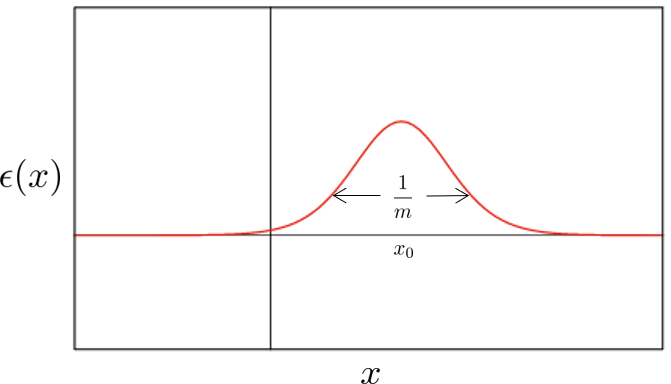
\includegraphics[width=10cm]{figure/fig2.png}
    \caption{}
    \label{fig2}
\end{figure}
そしてエネルギー密度を積分すればkink mass $M_\text{kink}$が得られ,
\begin{align*}
    M_{\text{kink}} & =\int_{-\infty}^{\infty}\mathrm{d}x~\epsilon(x)     \\
                    & =\dfrac{2\sqrt{2}}{3}\dfrac{m^3}{\lambda}           \\
                    & \Rightarrow \lambda \sim \dfrac{1}{M_{\text{kink}}}
\end{align*}
というようになり, 結合定数と質量の関係が得られる.

以上のように, 各模型に対して結合定数が定まっており, その値が1より非常に小さい場合, 結合定数の級数展開による摂動により模型を記述することができる. これをweak-coupling expansionと呼ぶ.


\begin{thebibliography}{99}
    \bibitem[morse] Morse, P. and Feshbach, H. (1953), "Methods of Mathematical Physics", McGraw-Hill Book Co., (New York).
\end{thebibliography}

\end{document}
